\section{Cache locality}

The principle of locality asserts that programs tend to access only a fraction of the total address space at any given moment. 
This principle is further elaborated through two key properties:
\begin{enumerate}
    \item \textit{Temporal locality}: if a memory location is accessed, it is probable that it will be accessed again in the near future.
    \item \textit{Spatial locality}: if a memory location is accessed, it is likely that nearby locations will also be accessed in the near future.
\end{enumerate}
Caches leverage both forms of locality. 
They exploit temporal locality by retaining the contents of recently accessed memory locations, anticipating their future use. 
Additionally, they exploit spatial locality by pre-fetching blocks of data surrounding recently accessed locations, capitalizing on the likelihood of adjacent memory access.

When examining a processor address, the cache tags are searched to locate a match. 
Subsequently, one of the following actions occurs:
\begin{itemize}
    \item \textit{Cache hit}: if a match is found in the cache, the data copy is retrieved from the cache and returned.
    \item \textit{Cache miss}: if the address is not found in the cache, a block of data is read from the main memory.
        There is a wait period, after which the data is returned to the processor, and the cache is updated accordingly.
\end{itemize}
Based on these operations, several metrics can be defined.
\begin{definition}[\textit{Hit rate}]
    The hit rate is the fraction of accesses that are found in the cache.
\end{definition}
\begin{definition}[\textit{Miss rate}]
    The miss rate is the complement of the hit rate, indicating the fraction of accesses that result in cache misses.
\end{definition}
\begin{definition}[\textit{Hit time}]
    The hit time comprises the time required for RAM access along with the time needed to determine whether the access resulted in a hit or miss.
\end{definition}
\begin{definition}[\textit{Miss time}]
    The miss time comprises the time necessary to replace a block in the cache and the time taken to deliver the block to the processor.
\end{definition}
\begin{figure}[H]
    \centering
    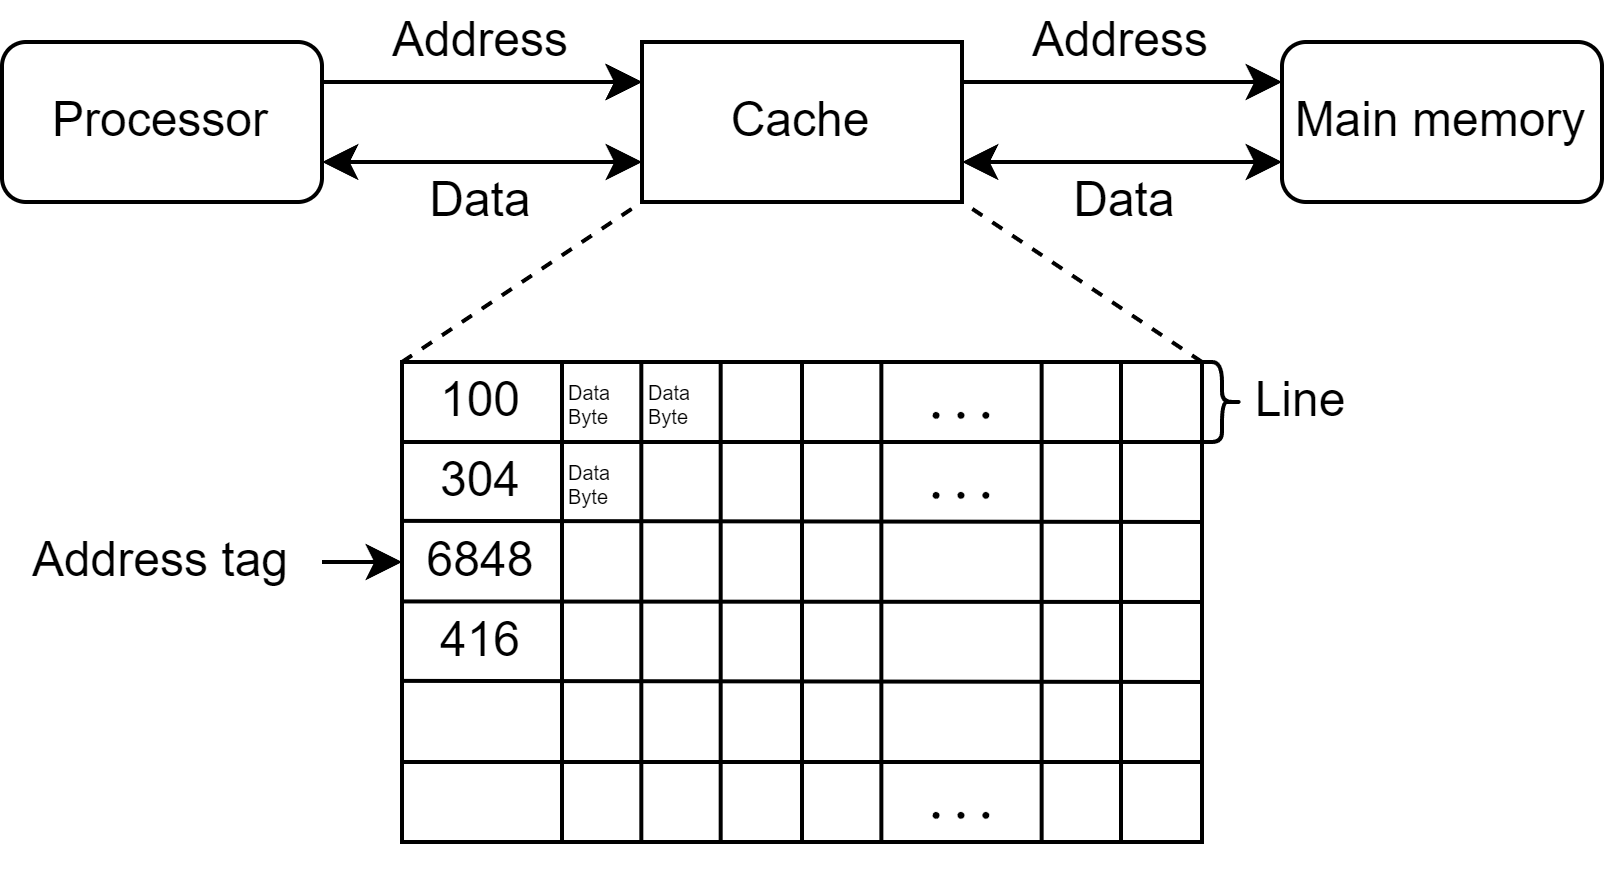
\includegraphics[width=0.5\linewidth]{images/cache.png}
    \caption{Cache and processor interaction}
\end{figure}

\subsection{Cache blocks}
Depending on the chosen cache type, the placement of a block number can be as follows:
\begin{itemize}
    \item \textit{Fully associative}: the block can be placed anywhere within the cache.
    \item \textit{Two-way set associative}: the block can be placed anywhere within set zero, which corresponds to $n \mod 4$.
    \item \textit{Direct mapped}: the block can only be placed into block four, determined by $n \mod 8$. 
\end{itemize}

\begin{figure}[H]
    \centering
    \begin{subfigure}{0.32\textwidth}
        \centering
        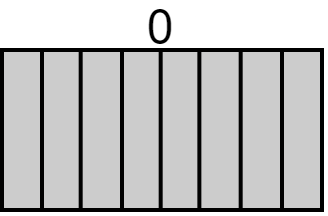
\includegraphics[width=0.45\linewidth]{images/fa.png} 
        \caption{Fully associative}
    \end{subfigure}
    \begin{subfigure}{0.32\textwidth}
        \centering
        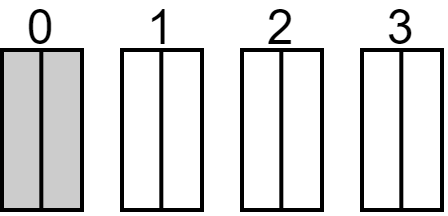
\includegraphics[width=0.6\linewidth]{images/twsa.png}
        \caption{Two-way set associative}
    \end{subfigure}
    \begin{subfigure}{0.32\textwidth}
        \centering
        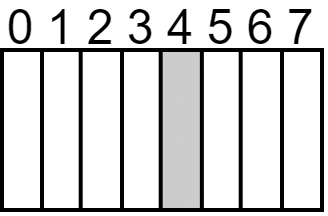
\includegraphics[width=0.45\linewidth]{images/dm.png}
        \caption{Direct mapped}
    \end{subfigure}
    \caption{Possible blocks placement}
\end{figure}

\subsection{Block read}
A cache miss can occur for several reasons:
\begin{enumerate}
    \item \textit{Compulsory miss} (cold start or process migration): this happens during the first access to a block, such as during a cold start or when a process migrates. 
        It's essentially an unavoidable aspect of system operation, and there's little that can be done to mitigate it.
    \item \textit{Capacity miss}: this occurs when the cache is unable to accommodate all the blocks accessed by the program. 
        Increasing the cache size can help reduce the frequency of these misses.
    \item \textit{Conflict miss} (collision): multiple memory locations are mapped to the same cache location, resulting in conflicts.
        This can be addressed by either increasing the cache size or increasing associativity, which allows more flexibility in mapping memory locations to cache locations.
    \item \textit{Coherence Miss} (invalidation): this type of miss occurs when another process, such as I/O operations, updates memory, leading to inconsistencies in cached data. 
        Ensuring cache coherence mechanisms are in place can help mitigate this issue.
\end{enumerate}
To locate a block, the cache index is used to select the set to search within, while the tag identifies the actual copy. 
If no matching candidates are found, a cache miss is declared.
The structure of a memory address typically includes a field for selecting data within a block.
\begin{figure}[H]
    \centering
    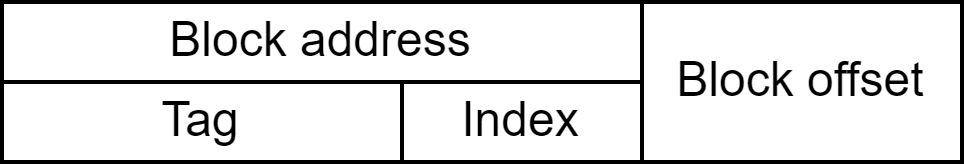
\includegraphics[width=0.5\linewidth]{images/address.png}
    \caption{Memory address general structure}
\end{figure}
Increasing associativity reduces the index size and expands the tag. 
Fully associative caches, for example, do not have an index field and can directly access any block in the cache.

The fully associative cache, characterized by requiring only a tag and block offset, is depicted as follows.
\begin{figure}[H]
    \centering
    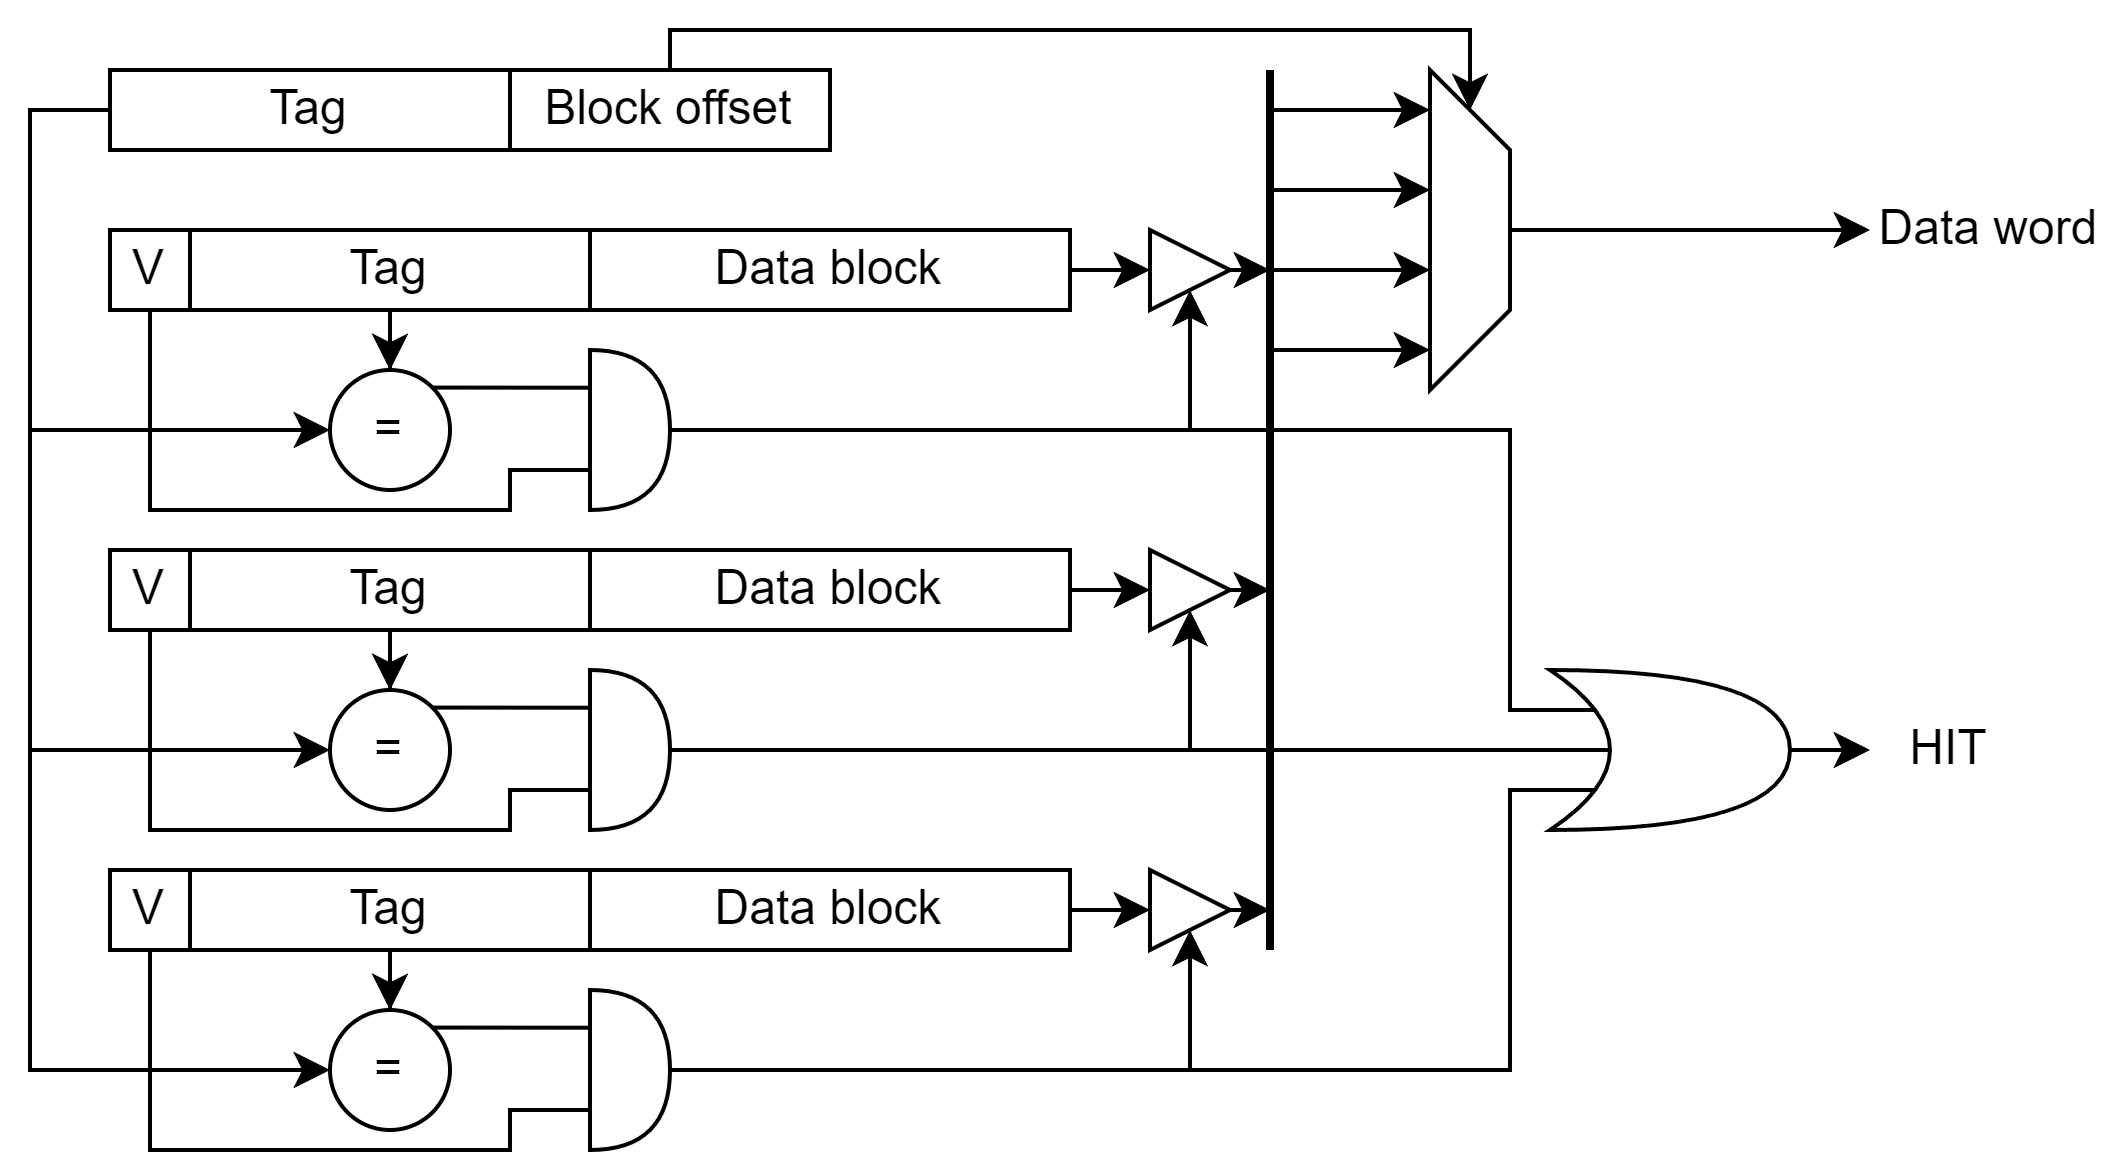
\includegraphics[width=0.75\linewidth]{images/fas.png} 
    \caption{Fully associative cache}
\end{figure}
The two-way set associative cache, which necessitates a tag, index, and block offset, is represented as follows.
\begin{figure}[H]
    \centering
    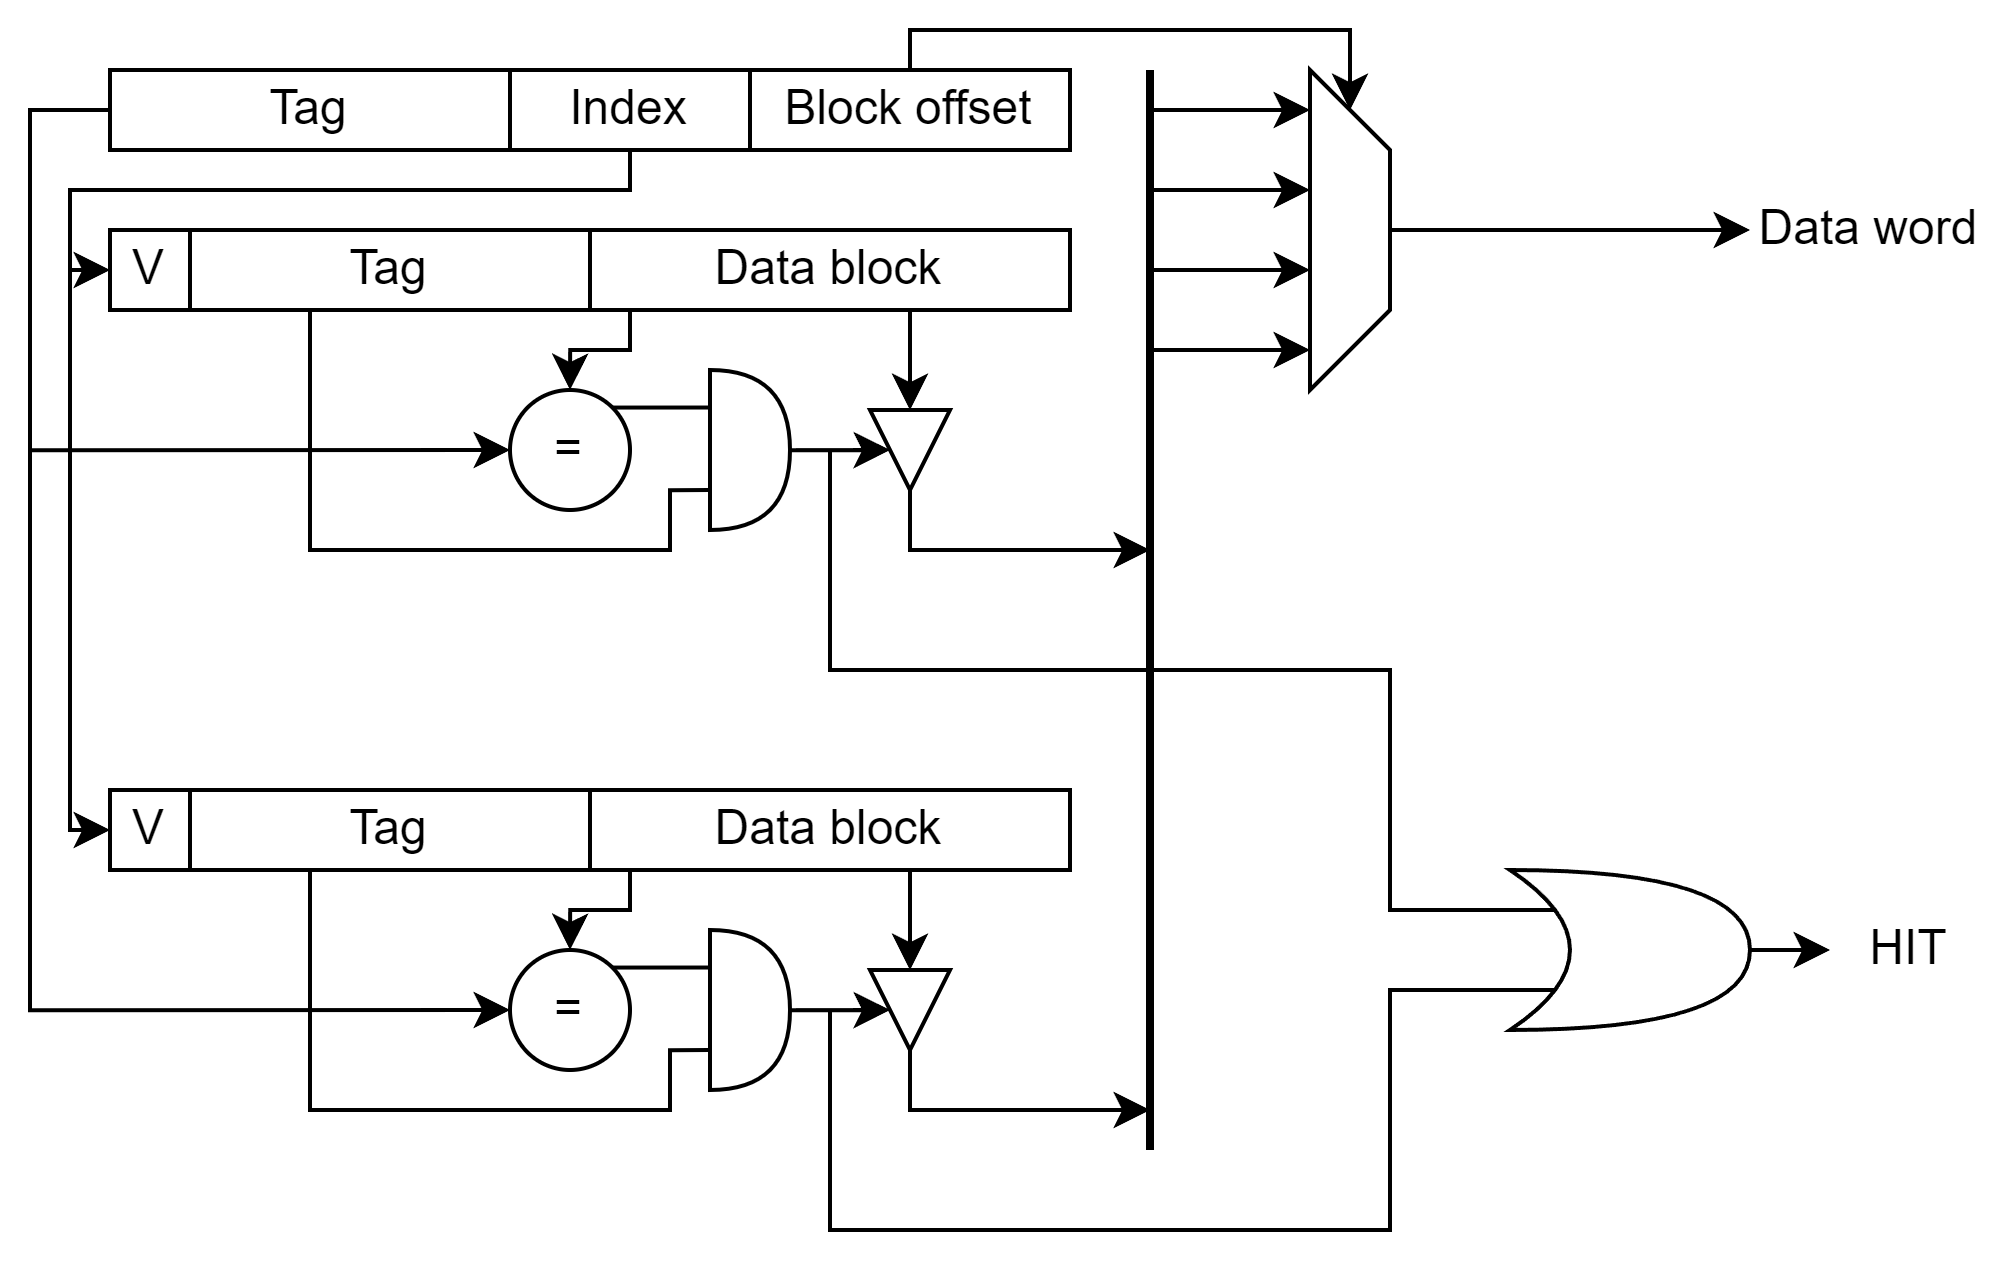
\includegraphics[width=0.75\linewidth]{images/twsas.png}
    \caption{Two-way set associative cache}
\end{figure}
The direct-mapped cache, which also requires a tag, index, and block offset, is illustrated as follows.
\begin{figure}[H]
    \centering
    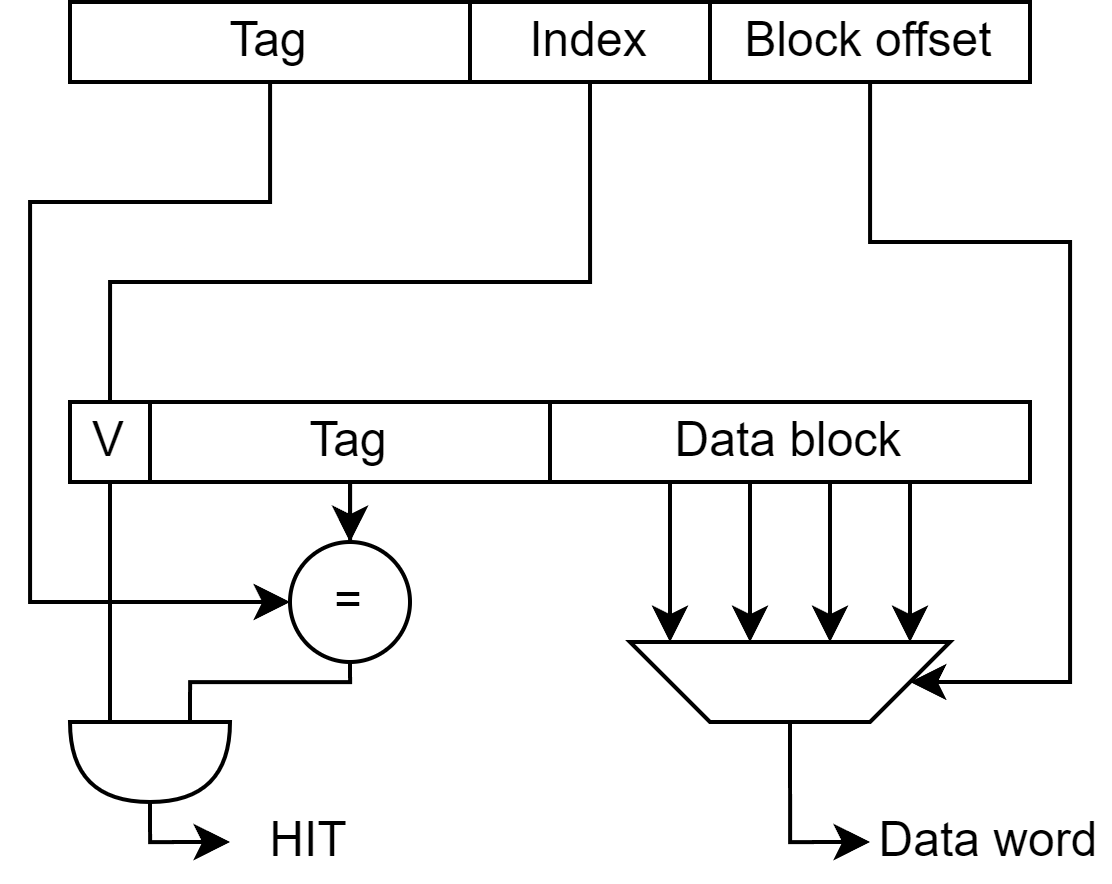
\includegraphics[width=0.5\linewidth]{images/dms.png}
    \caption{Direct mapped cache}
\end{figure}

\subsection{Block replacement}
In the context of cache misses, block replacement is straightforward for direct-mapped caches. 
However, for set-associative or fully associative caches, the choice of replacement policy has a significant impact since replacements only occur upon misses. 
Here are some commonly used replacement policies:
\begin{itemize}
    \item \textit{Random}: blocks are replaced randomly, without any specific order or pattern.
    \item \textit{Least Recently Used} (LRU): this policy replaces the block that has been accessed least recently. 
        Although effective, implementing LRU requires tracking the access history of each block, making it feasible only for caches with a few sets due to the computational overhead.
    \item \textit{First In First Out} (FIFO): blocks are replaced based on the order they were brought into the cache. 
        FIFO is commonly used in highly associative caches where keeping track of access history for LRU may not be practical.
\end{itemize}

\subsection{Block write}
When handling writes, we have two main options for a cache hit:
\begin{itemize}
    \item \textit{Write through}: this strategy involves writing the data both to the cache and to main memory simultaneously. 
        While this approach typically results in higher traffic, it simplifies cache coherence management.
    \item \textit{Write back}: with this approach, data is written only to the cache. 
        The corresponding entry in main memory is updated only when the cache block is evicted. 
        A dirty bit per block helps reduce traffic by indicating whether the block in the cache has been modified.
\end{itemize}
In the case of a cache miss, there are two alternatives:
\begin{itemize}
    \item \textit{No write allocate}: data is written directly to main memory without being fetched into the cache.
    \item \textit{Write allocate}: in this scenario, the data is fetched into the cache upon a write miss.
\end{itemize}
The most common combinations of these strategies are:
\begin{itemize}
    \item \textit{Write through with no write allocate}: data is written to both the cache and main memory simultaneously. In the event of a write miss, no data is brought into the cache.
    \item \textit{Write back with write allocate}: data is written only to the cache, and in the case of a write miss, the data is fetched into the cache before being modified.
\end{itemize}
Additionally, a write buffer can be used for write-through caches to avoid CPU stalls.